
%% bare_jrnl.tex
%% V1.3
%% 2007/01/11
%% by Michael Shell
%% see http://www.michaelshell.org/
%% for current contact information.
%%
%% This is a skeleton file demonstrating the use of IEEEtran.cls
%% (requires IEEEtran.cls version 1.7 or later) with an IEEE journal paper.
%%
%% Support sites:
%% http://www.michaelshell.org/tex/ieeetran/
%% http://www.ctan.org/tex-archive/macros/latex/contrib/IEEEtran/
%% and
%% http://www.ieee.org/



% *** Authors should verify (and, if needed, correct) their LaTeX system  ***
% *** with the testflow diagnostic prior to trusting their LaTeX platform ***
% *** with production work. IEEE's font choices can trigger bugs that do  ***
% *** not appear when using other class files.                            ***
% The testflow support page is at:
% http://www.michaelshell.org/tex/testflow/


%%*************************************************************************
%% Legal Notice:
%% This code is offered as-is without any warranty either expressed or
%% implied; without even the implied warranty of MERCHANTABILITY or
%% FITNESS FOR A PARTICULAR PURPOSE! 
%% User assumes all risk.
%% In no event shall IEEE or any contributor to this code be liable for
%% any damages or losses, including, but not limited to, incidental,
%% consequential, or any other damages, resulting from the use or misuse
%% of any information contained here.
%%
%% All comments are the opinions of their respective authors and are not
%% necessarily endorsed by the IEEE.
%%
%% This work is distributed under the LaTeX Project Public License (LPPL)
%% ( http://www.latex-project.org/ ) version 1.3, and may be freely used,
%% distributed and modified. A copy of the LPPL, version 1.3, is included
%% in the base LaTeX documentation of all distributions of LaTeX released
%% 2003/12/01 or later.
%% Retain all contribution notices and credits.
%% ** Modified files should be clearly indicated as such, including  **
%% ** renaming them and changing author support contact information. **
%%
%% File list of work: IEEEtran.cls, IEEEtran_HOWTO.pdf, bare_adv.tex,
%%                    bare_conf.tex, bare_jrnl.tex, bare_jrnl_compsoc.tex
%%*************************************************************************

% Note that the a4paper option is mainly intended so that authors in
% countries using A4 can easily print to A4 and see how their papers will
% look in print - the typesetting of the document will not typically be
% affected with changes in paper size (but the bottom and side margins will).
% Use the testflow package mentioned above to verify correct handling of
% both paper sizes by the user's LaTeX system.
%
% Also note that the "draftcls" or "draftclsnofoot", not "draft", option
% should be used if it is desired that the figures are to be displayed in
% draft mode.
%
\documentclass[journal]{IEEEtran}
%
% If IEEEtran.cls has not been installed into the LaTeX system files,
% manually specify the path to it like:
% \documentclass[journal]{../sty/IEEEtran}





% Some very useful LaTeX packages include:
% (uncomment the ones you want to load)


% *** MISC UTILITY PACKAGES ***
%
%\usepackage{ifpdf}
% Heiko Oberdiek's ifpdf.sty is very useful if you need conditional
% compilation based on whether the output is pdf or dvi.
% usage:
% \ifpdf
%   % pdf code
% \else
%   % dvi code
% \fi
% The latest version of ifpdf.sty can be obtained from:
% http://www.ctan.org/tex-archive/macros/latex/contrib/oberdiek/
% Also, note that IEEEtran.cls V1.7 and later provides a builtin
% \ifCLASSINFOpdf conditional that works the same way.
% When switching from latex to pdflatex and vice-versa, the compiler may
% have to be run twice to clear warning/error messages.






% *** CITATION PACKAGES ***
%
%\usepackage{cite}
% cite.sty was written by Donald Arseneau
% V1.6 and later of IEEEtran pre-defines the format of the cite.sty package
% \cite{} output to follow that of IEEE. Loading the cite package will
% result in citation numbers being automatically sorted and properly
% "compressed/ranged". e.g., [1], [9], [2], [7], [5], [6] without using
% cite.sty will become [1], [2], [5]--[7], [9] using cite.sty. cite.sty's
% \cite will automatically add leading space, if needed. Use cite.sty's
% noadjust option (cite.sty V3.8 and later) if you want to turn this off.
% cite.sty is already installed on most LaTeX systems. Be sure and use
% version 4.0 (2003-05-27) and later if using hyperref.sty. cite.sty does
% not currently provide for hyperlinked citations.
% The latest version can be obtained at:
% http://www.ctan.org/tex-archive/macros/latex/contrib/cite/
% The documentation is contained in the cite.sty file itself.






% *** GRAPHICS RELATED PACKAGES ***
%
\ifCLASSINFOpdf
\usepackage[pdftex]{graphicx}
  % declare the path(s) where your graphic files are
  % \graphicspath{{../pdf/}{../jpeg/}}
  % and their extensions so you won't have to specify these with
  % every instance of \includegraphics
  % \DeclareGraphicsExtensions{.pdf,.jpeg,.png}
\else
  % or other class option (dvipsone, dvipdf, if not using dvips). graphicx
  % will default to the driver specified in the system graphics.cfg if no
  % driver is specified.
\usepackage[dvips]{graphicx}
  % declare the path(s) where your graphic files are
  % \graphicspath{{../eps/}}
  % and their extensions so you won't have to specify these with
  % every instance of \includegraphics
  % \DeclareGraphicsExtensions{.eps}
\fi
% graphicx was written by David Carlisle and Sebastian Rahtz. It is
% required if you want graphics, photos, etc. graphicx.sty is already
% installed on most LaTeX systems. The latest version and documentation can
% be obtained at: 
% http://www.ctan.org/tex-archive/macros/latex/required/graphics/
% Another good source of documentation is "Using Imported Graphics in
% LaTeX2e" by Keith Reckdahl which can be found as epslatex.ps or
% epslatex.pdf at: http://www.ctan.org/tex-archive/info/
%
% latex, and pdflatex in dvi mode, support graphics in encapsulated
% postscript (.eps) format. pdflatex in pdf mode supports graphics
% in .pdf, .jpeg, .png and .mps (metapost) formats. Users should ensure
% that all non-photo figures use a vector format (.eps, .pdf, .mps) and
% not a bitmapped formats (.jpeg, .png). IEEE frowns on bitmapped formats
% which can result in "jaggedy"/blurry rendering of lines and letters as
% well as large increases in file sizes.
%
% You can find documentation about the pdfTeX application at:
% http://www.tug.org/applications/pdftex





% *** MATH PACKAGES ***
%
\usepackage[cmex10]{amsmath}
% A popular package from the American Mathematical Society that provides
% many useful and powerful commands for dealing with mathematics. If using
% it, be sure to load this package with the cmex10 option to ensure that
% only type 1 fonts will utilized at all point sizes. Without this option,
% it is possible that some math symbols, particularly those within
% footnotes, will be rendered in bitmap form which will result in a
% document that can not be IEEE Xplore compliant!
%
% Also, note that the amsmath package sets \interdisplaylinepenalty to 10000
% thus preventing page breaks from occurring within multiline equations. Use:
%\interdisplaylinepenalty=2500
% after loading amsmath to restore such page breaks as IEEEtran.cls normally
% does. amsmath.sty is already installed on most LaTeX systems. The latest
% version and documentation can be obtained at:
% http://www.ctan.org/tex-archive/macros/latex/required/amslatex/math/





% *** SPECIALIZED LIST PACKAGES ***
%
\usepackage{algorithmic}
% algorithmic.sty was written by Peter Williams and Rogerio Brito.
% This package provides an algorithmic environment fo describing algorithms.
% You can use the algorithmic environment in-text or within a figure
% environment to provide for a floating algorithm. Do NOT use the algorithm
% floating environment provided by algorithm.sty (by the same authors) or
% algorithm2e.sty (by Christophe Fiorio) as IEEE does not use dedicated
% algorithm float types and packages that provide these will not provide
% correct IEEE style captions. The latest version and documentation of
% algorithmic.sty can be obtained at:
% http://www.ctan.org/tex-archive/macros/latex/contrib/algorithms/
% There is also a support site at:
% http://algorithms.berlios.de/index.html
% Also of interest may be the (relatively newer and more customizable)
% algorithmicx.sty package by Szasz Janos:
% http://www.ctan.org/tex-archive/macros/latex/contrib/algorithmicx/




% *** ALIGNMENT PACKAGES ***
%
\usepackage{array}
% Frank Mittelbach's and David Carlisle's array.sty patches and improves
% the standard LaTeX2e array and tabular environments to provide better
% appearance and additional user controls. As the default LaTeX2e table
% generation code is lacking to the point of almost being broken with
% respect to the quality of the end results, all users are strongly
% advised to use an enhanced (at the very least that provided by array.sty)
% set of table tools. array.sty is already installed on most systems. The
% latest version and documentation can be obtained at:
% http://www.ctan.org/tex-archive/macros/latex/required/tools/


%\usepackage{mdwmath}
%\usepackage{mdwtab}
% Also highly recommended is Mark Wooding's extremely powerful MDW tools,
% especially mdwmath.sty and mdwtab.sty which are used to format equations
% and tables, respectively. The MDWtools set is already installed on most
% LaTeX systems. The lastest version and documentation is available at:
% http://www.ctan.org/tex-archive/macros/latex/contrib/mdwtools/


% IEEEtran contains the IEEEeqnarray family of commands that can be used to
% generate multiline equations as well as matrices, tables, etc., of high
% quality.


%\usepackage{eqparbox}
% Also of notable interest is Scott Pakin's eqparbox package for creating
% (automatically sized) equal width boxes - aka "natural width parboxes".
% Available at:
% http://www.ctan.org/tex-archive/macros/latex/contrib/eqparbox/





% *** SUBFIGURE PACKAGES ***
%\usepackage[tight,footnotesize]{subfigure}
% subfigure.sty was written by Steven Douglas Cochran. This package makes it
% easy to put subfigures in your figures. e.g., "Figure 1a and 1b". For IEEE
% work, it is a good idea to load it with the tight package option to reduce
% the amount of white space around the subfigures. subfigure.sty is already
% installed on most LaTeX systems. The latest version and documentation can
% be obtained at:
% http://www.ctan.org/tex-archive/obsolete/macros/latex/contrib/subfigure/
% subfigure.sty has been superceeded by subfig.sty.



%\usepackage[caption=false]{caption}
%\usepackage[font=footnotesize]{subfig}
% subfig.sty, also written by Steven Douglas Cochran, is the modern
% replacement for subfigure.sty. However, subfig.sty requires and
% automatically loads Axel Sommerfeldt's caption.sty which will override
% IEEEtran.cls handling of captions and this will result in nonIEEE style
% figure/table captions. To prevent this problem, be sure and preload
% caption.sty with its "caption=false" package option. This is will preserve
% IEEEtran.cls handing of captions. Version 1.3 (2005/06/28) and later 
% (recommended due to many improvements over 1.2) of subfig.sty supports
% the caption=false option directly:
%\usepackage[caption=false,font=footnotesize]{subfig}
%
% The latest version and documentation can be obtained at:
% http://www.ctan.org/tex-archive/macros/latex/contrib/subfig/
% The latest version and documentation of caption.sty can be obtained at:
% http://www.ctan.org/tex-archive/macros/latex/contrib/caption/




% *** FLOAT PACKAGES ***
%
%\usepackage{fixltx2e}
% fixltx2e, the successor to the earlier fix2col.sty, was written by
% Frank Mittelbach and David Carlisle. This package corrects a few problems
% in the LaTeX2e kernel, the most notable of which is that in current
% LaTeX2e releases, the ordering of single and double column floats is not
% guaranteed to be preserved. Thus, an unpatched LaTeX2e can allow a
% single column figure to be placed prior to an earlier double column
% figure. The latest version and documentation can be found at:
% http://www.ctan.org/tex-archive/macros/latex/base/



%\usepackage{stfloats}
% stfloats.sty was written by Sigitas Tolusis. This package gives LaTeX2e
% the ability to do double column floats at the bottom of the page as well
% as the top. (e.g., "\begin{figure*}[!b]" is not normally possible in
% LaTeX2e). It also provides a command:
%\fnbelowfloat
% to enable the placement of footnotes below bottom floats (the standard
% LaTeX2e kernel puts them above bottom floats). This is an invasive package
% which rewrites many portions of the LaTeX2e float routines. It may not work
% with other packages that modify the LaTeX2e float routines. The latest
% version and documentation can be obtained at:
% http://www.ctan.org/tex-archive/macros/latex/contrib/sttools/
% Documentation is contained in the stfloats.sty comments as well as in the
% presfull.pdf file. Do not use the stfloats baselinefloat ability as IEEE
% does not allow \baselineskip to stretch. Authors submitting work to the
% IEEE should note that IEEE rarely uses double column equations and
% that authors should try to avoid such use. Do not be tempted to use the
% cuted.sty or midfloat.sty packages (also by Sigitas Tolusis) as IEEE does
% not format its papers in such ways.


%\ifCLASSOPTIONcaptionsoff
%  \usepackage[nomarkers]{endfloat}
% \let\MYoriglatexcaption\caption
% \renewcommand{\caption}[2][\relax]{\MYoriglatexcaption[#2]{#2}}
%\fi
% endfloat.sty was written by James Darrell McCauley and Jeff Goldberg.
% This package may be useful when used in conjunction with IEEEtran.cls'
% captionsoff option. Some IEEE journals/societies require that submissions
% have lists of figures/tables at the end of the paper and that
% figures/tables without any captions are placed on a page by themselves at
% the end of the document. If needed, the draftcls IEEEtran class option or
% \CLASSINPUTbaselinestretch interface can be used to increase the line
% spacing as well. Be sure and use the nomarkers option of endfloat to
% prevent endfloat from "marking" where the figures would have been placed
% in the text. The two hack lines of code above are a slight modification of
% that suggested by in the endfloat docs (section 8.3.1) to ensure that
% the full captions always appear in the list of figures/tables - even if
% the user used the short optional argument of \caption[]{}.
% IEEE papers do not typically make use of \caption[]'s optional argument,
% so this should not be an issue. A similar trick can be used to disable
% captions of packages such as subfig.sty that lack options to turn off
% the subcaptions:
% For subfig.sty:
% \let\MYorigsubfloat\subfloat
% \renewcommand{\subfloat}[2][\relax]{\MYorigsubfloat[]{#2}}
% For subfigure.sty:
% \let\MYorigsubfigure\subfigure
% \renewcommand{\subfigure}[2][\relax]{\MYorigsubfigure[]{#2}}
% However, the above trick will not work if both optional arguments of
% the \subfloat/subfig command are used. Furthermore, there needs to be a
% description of each subfigure *somewhere* and endfloat does not add
% subfigure captions to its list of figures. Thus, the best approach is to
% avoid the use of subfigure captions (many IEEE journals avoid them anyway)
% and instead reference/explain all the subfigures within the main caption.
% The latest version of endfloat.sty and its documentation can obtained at:
% http://www.ctan.org/tex-archive/macros/latex/contrib/endfloat/
%
% The IEEEtran \ifCLASSOPTIONcaptionsoff conditional can also be used
% later in the document, say, to conditionally put the References on a 
% page by themselves.





% *** PDF, URL AND HYPERLINK PACKAGES ***
%
%\usepackage{url}
% url.sty was written by Donald Arseneau. It provides better support for
% handling and breaking URLs. url.sty is already installed on most LaTeX
% systems. The latest version can be obtained at:
% http://www.ctan.org/tex-archive/macros/latex/contrib/misc/
% Read the url.sty source comments for usage information. Basically,
% \url{my_url_here}.





% *** Do not adjust lengths that control margins, column widths, etc. ***
% *** Do not use packages that alter fonts (such as pslatex).         ***
% There should be no need to do such things with IEEEtran.cls V1.6 and later.
% (Unless specifically asked to do so by the journal or conference you plan
% to submit to, of course. )





%%%%%%%%%%%%%%%%%%%%%%%%%%%%%%%%%%%%%%%%%%%%%
%%%%%%%%%      PACKAGES INTRODUCED BY US      %%%%%%%%%

%for the copyright
\usepackage{textcomp}







% correct bad hyphenation here
\hyphenation{op-tical net-works semi-conduc-tor}


\begin{document}
%
% paper title
% can use linebreaks \\ within to get better formatting as desired
\title{Optimized navigation behaviour of multiple robots based on motor-schema}
%
%
% author names and IEEE memberships
% note positions of commas and nonbreaking spaces ( ~ ) LaTeX will not break
% a structure at a ~ so this keeps an author's name from being broken across
% two lines.
% use \thanks{} to gain access to the first footnote area
% a separate \thanks must be used for each paragraph as LaTeX2e's \thanks
% was not built to handle multiple paragraphs
%

\author{Ondine~Chanon,~\IEEEmembership{CSE},
        Nicolas~Hubacher,~\IEEEmembership{IN},
        Stefano~Savar\`e,~\IEEEmembership{CSE}}% <-this % stops a space
%\thanks{M. Shell is with the Department
%of Electrical and Computer Engineering, Georgia Institute of Technology, Atlanta,
%GA, 30332 USA e-mail: (see http://www.michaelshell.org/contact.html).}% <-this % stops a space
%\thanks{J. Doe and J. Doe are with Anonymous University.}% <-this % stops a space
%\thanks{Manuscript received April 19, 2005; revised January 11, 2007.}}

% note the % following the last \IEEEmembership and also \thanks - 
% these prevent an unwanted space from occurring between the last author name
% and the end of the author line. i.e., if you had this:
% 
% \author{....lastname \thanks{...} \thanks{...} }
%                     ^------------^------------^----Do not want these spaces!
%
% a space would be appended to the last name and could cause every name on that
% line to be shifted left slightly. This is one of those "LaTeX things". For
% instance, "\textbf{A} \textbf{B}" will typeset as "A B" not "AB". To get
% "AB" then you have to do: "\textbf{A}\textbf{B}"
% \thanks is no different in this regard, so shield the last } of each \thanks
% that ends a line with a % and do not let a space in before the next \thanks.
% Spaces after \IEEEmembership other than the last one are OK (and needed) as
% you are supposed to have spaces between the names. For what it is worth,
% this is a minor point as most people would not even notice if the said evil
% space somehow managed to creep in.



% The paper headers
\markboth{Distributed Intelligent System, Course Project, December 2015}%
{Shell \MakeLowercase{\textit{et al.}}: Bare Demo of IEEEtran.cls for Journals}
% The only time the second header will appear is for the odd numbered pages
% after the title page when using the twoside option.
% 
% *** Note that you probably will NOT want to include the author's ***
% *** name in the headers of peer review papers.                   ***
% You can use \ifCLASSOPTIONpeerreview for conditional compilation here if
% you desire.




% If you want to put a publisher's ID mark on the page you can do it like
% this:
%\IEEEpubid{0000--0000/00\$00.00~\copyright~2007 IEEE}
% Remember, if you use this you must call \IEEEpubidadjcol in the second
% column for its text to clear the IEEEpubid mark.



% use for special paper notices
%\IEEEspecialpapernotice{(Invited Paper)}




% make the title area
\maketitle


%\begin{abstract}
%%\boldmath
%The abstract goes here.
%\end{abstract}
%% IEEEtran.cls defaults to using nonbold math in the Abstract.
%% This preserves the distinction between vectors and scalars. However,
%% if the journal you are submitting to favors bold math in the abstract,
%% then you can use LaTeX's standard command \boldmath at the very start
%% of the abstract to achieve this. Many IEEE journals frown on math
%% in the abstract anyway.
%
%% Note that keywords are not normally used for peerreview papers.
%\begin{IEEEkeywords}
%IEEEtran, journal, \LaTeX, paper, template.
%\end{IEEEkeywords}






% For peer review papers, you can put extra information on the cover
% page as needed:
% \ifCLASSOPTIONpeerreview
% \begin{center} \bfseries EDICS Category: 3-BBND \end{center}
% \fi
%
% For peerreview papers, this IEEEtran command inserts a page break and
% creates the second title. It will be ignored for other modes.
\IEEEpeerreviewmaketitle

\section*{Abstract}
Motor schemas are among the main techniques that allow navigation
of mobile robots in complex worlds full of obstacles. However,
as the number of schemas and the complexity increase, it may be very
difficult and time expensive to tune correctly all the parameters that
rule the simulation. The introduction of some machine learning
techniques (in our case Particle Swarm Optimization) thus becomes necessary. 
\textbf{TODO: Add a paragraph with the results.}


\section{Introduction}
\label {sec:1}
% The very first letter is a 2 line initial drop letter followed
% by the rest of the first word in caps.
% 
% form to use if the first word consists of a single letter:
% \IEEEPARstart{A}{demo} file is ....
% 
% form to use if you need the single drop letter followed by
% normal text (unknown if ever used by IEEE):
% \IEEEPARstart{A}{}demo file is ....
% 
% Some journals put the first two words in caps:
% \IEEEPARstart{T}{his demo} file is ....
% 
% Here we have the typical use of a "T" for an initial drop letter
% and "HIS" in caps to complete the first word.
\IEEEPARstart{T}{he} first aim of the project was to implement a controller
for mobile robots (e-puck in our case) based on motor schemas, and test it with simulations
using the software
Webots\textregistered. \cite{IEEEhowto:arkin_motor_schemas} and 
\cite{IEEEhowto:balch_behaviour_based} provide a
good explanation of the purpose of motor-schema based
controllers over traditional and less flexible ones. One of the main challenges that one may encounter while implementing the controller
is to achieve multiple different objectives at the same time,
to obtain an optimised and good looking walk of the robots. 
Motor schemas provide an elegant way to do so: at each instant, the
robots compute a different speed vector for each objective and then
sum them all with appropriate weights. 
The robots in our case should move in an environment full of obstacles while
keeping a precise formation, avoiding other robots and moving towards
a goal. We will show in section \ref{sec:2} how we implemented such behaviour.

Tuning correctly the motor-schemas parameters leads to the second part of our project:
we studied the influence on the simulation of Particle Swarm Optimization (PSO), a
powerful machine learning technique. Indeed, it is difficult to manually set the parameters even with just a few ones, and it becomes almost impossible as their
number increases. PSO (see \cite{IEEEhowto:martinoli_pso},
\cite{IEEEhowto:martinoli_pso_noise}, \cite{IEEEhowto:martinoli_pso_noise_2}) is a recent and promising technique that, in short, consists in modelling the set of potential problem solutions as a swarm of particles moving around in a virtual multi-dimensional
search space. 
% TODO: how much about PSO do we want to mention in the intro, how much later?
Each particle, after being evaluated, moves keeping in memory its neighbourhood's and its own best positions acquired so far. Ideally, the particles should converge to a global optimal position. 

PSO can model an Artificial Neural Network controller: the parameter set contains the weights and, with appropriate extensions and taking into account the noise, this method suits perfectly the robot swarm problem.  
A key part of PSO is the choice of a good fitness function to evaluate the performance of each parameter set. A good reference fitness function is the one of Floreano and Mondada \cite{IEEEhowto:fitness_floreano_mondada}. Based on this, we have developed our own fitness function that will be explained in section \ref{sec:3}. 

In section \ref{sec:4}, we will present the results of our
simulations and the final section \ref{sec:5} will be reserved to our conclusions. 
\textbf{TODO: maybe add something on the setting of our simulations and future work}

\section{Motor-schemas}
\label{sec:2}
\IEEEPARstart{W}{e} have considered five basic motor schemas: \textit{move to goal}, \textit{keep formation}, \textit{avoid other robots}, \textit{avoid obstacles}, and \textit{random walk}. % described below:
%\begin{itemize}
%\item \textit{Move to goal}
%\item \textit{Keep formation}
%\item \textit{Avoid other robots}
%\item \textit{Avoid obstacles}
%\item \textit{Random walk}
%\end{itemize}
Each schema provides a normalized speed vector (with norm between
0 and 1). All of these contributions are then summed with appropriate weights, obtaining the
global speed vector which will determine the wheel speeds of the robots. 
Excluding the fifth schema, all the other ones use the concept of
\textit{Sphere of Influence} as proposed in
\cite{IEEEhowto:arkin_motor_schemas}. The idea is that the cause of a
behaviour influences the robot only if its value is lower (or higher, depending on the behaviour) than a certain value $S$ (the radius of the sphere of influence). We can extend this concept considering two thresholds $R$ and $S$: the reaction will be maximum (or minimum) if the value is below $R$ and minimum (or maximum) if it is higher than $S$. Between $R$ and $S$ we usually adopt a linear behaviour, even if more complex equations can be considered.

To compute all the necessary information, the robots can communicate with a supervisor that sends them their own position (not the ones of the other robots) and the goal position. They can also communicate with the other robots which are not too far away in order to exchange their relative position. They moreover use their infra-red based distance sensors to detect obstacles.

\subsection{Move to goal}  
The simplest motor schema is the \textit{move to goal} one. Knowing the positions of the robots and the position of the goal (communicated by the supervisor), this schema generates a speed vector $d_{goal}$ with a direction from the unit center of the flock to the goal and of norm $|d_{goal}|$. We have:
\begin{equation}
|d_{goal}| = \begin{cases} 0, & \mbox{if }  d<R \\ \frac{d-R}{S-R}, & \mbox{if }
   R<d<S \\ 1 & \mbox{if } d>S\end{cases}
\end{equation}
where $d$ is the distance between the unit center and the goal. The unit center is computed through local communication.

\subsection{Keep formation}
The \textit{keep formation} schema is conceptually similar to the move to goal schema. The difference is that the goal does now correspond to the position in which the robot should be in order to stay in formation and that it has to be computed at each time step. Knowing the position of the goal, the unit center of the formation, and the coordinates of each robot relatively to the unit center, it is possible to compute the vector from the actual position to the expected one (see Figure \ref{img:keep_formation}). 
\begin{figure}[!t]
\centering
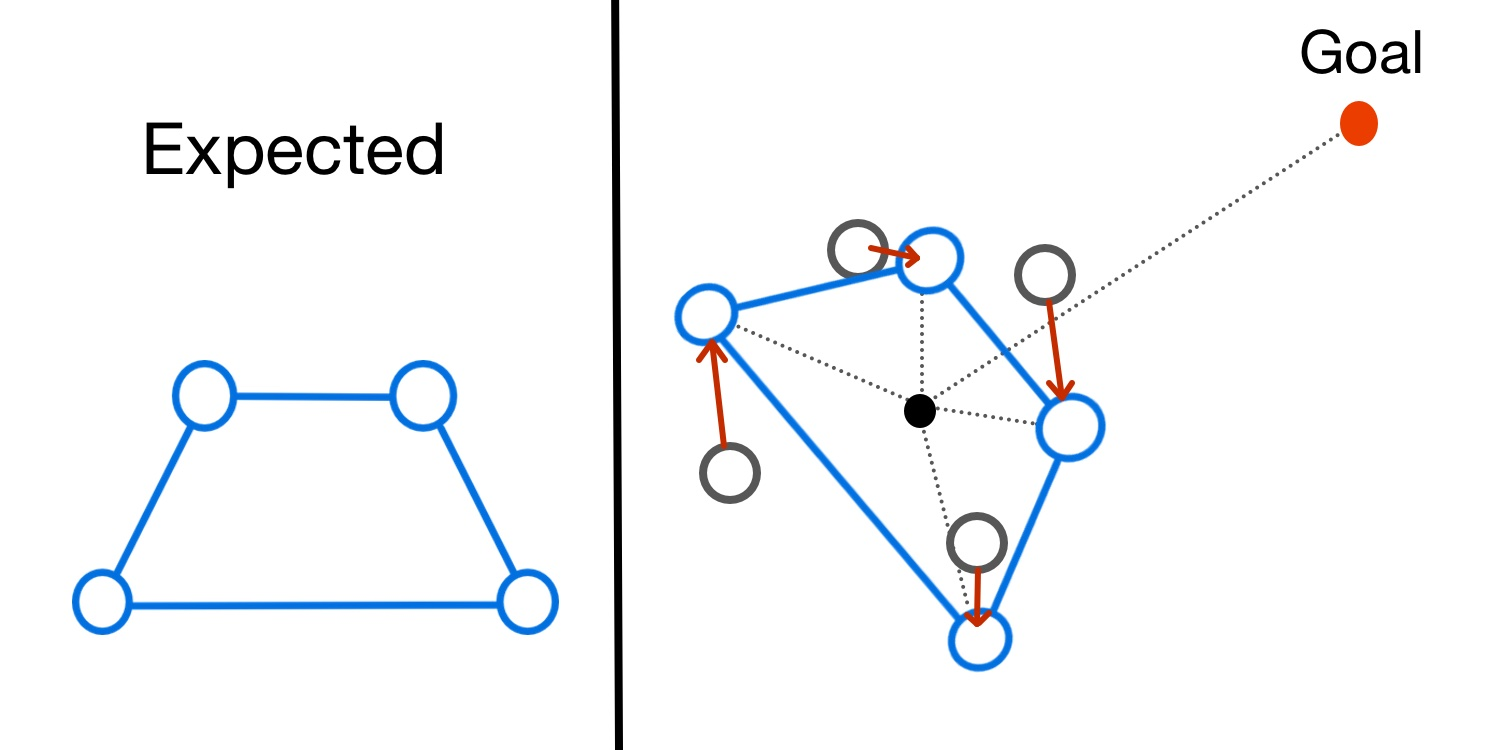
\includegraphics[width=3.5in]{Images/keep_formation.jpg}
\caption{Computation of the expected position in the keep formation motor schema}
\label{img:keep_formation}
\end{figure}

\subsection{Avoid other robots}
To detect the other robots, we can either use the built-in sensors, or local communication. We decided to use the second variant since we found it much more precise and less noisy than sensor values. Once implemented local communications, the robots can easily receive the
positions of the other robots. For each robots, a speed vector is generated, pointing outward the other robot and having the following norm:
\begin{equation}
\begin{cases} 1, & \mbox{if }  d<R \\ \frac{S-d}{S-R}, & \mbox{if }
  R<d<S \\ 0 & \mbox{if } d>S\end{cases}
\end{equation}
where $d$ is the distance between the two robots. Then all the generated vectors
are summed. Note that the formula is the opposite to the one in the
\textit{move to goal} scheme, since in this case we want to avoid an object
instead of moving towards it.

\subsection{Avoid obstacles}
There are eight infra-red distance sensors on an e-puck and we know the position and thus the orientation of each of them. Now, $R$ and $S$ are sensor values: if the received sensor value is below $R$, we assume that no obstacle is near; if it is over $S$, we generate a normalized vector in the opposite direction. 

Since the sensor values are very noisy, we have decided to work with a moving average. Through an empirical analysis we came to the conclusion that a perception window size of $2$ is a good choice. We thus use each sensor's current and last value for the computation of the average. Furthermore, in order to increase the influence of high sensor values (representing a short distance to a certain object), we double their weight for the computation of the average. Thanks to this technique, the robots behave more smoothly. The final speed vector is computed as the sum of the vectors relative to each sensor.

\subsection{Random walk}
The four previous motor schemas are theoretically sufficient to achieve the goals of our project, but the presence of noise often creates a tricky evaluation. Moreover, some difficult obstacle configurations are hard to get over considering only these previously presented schemas. One possible solution to improve the performance is to add a random component to the speed of the robots. This is usually a bad idea in absence of obstacles since it creates a smooth fluid walk, but in our situation, if a robot is stuck behind an obstacle this additional random component can possibly free the robot by leading it towards a random direction.
There are many ways of adding noise, our implementation is based on two
components:
\begin{itemize}
\item \textit{Noise generation frequency:} this determines how often the noise vector should be recomputed. A higher number would help a robot escape more easily after getting stuck behind an obstacle, while a lower value would allow a smoother walk towards the goal.
\item \textit{Fading:} At each re-computation, the vector is computed as a linear combination of a completely new random vector and the one previously computed. This helps provide a more natural walk without sudden changes of direction.
\end{itemize}

% You must have at least 2 lines in the paragraph with the drop letter
% (should never be an issue)


%\subsection{Subsection Heading Here}
%Subsection text here.

% needed in second column of first page if using \IEEEpubid
%\IEEEpubidadjcol

%\subsubsection{Subsubsection Heading Here}
%Subsubsection text here.


% An example of a floating figure using the graphicx package.
% Note that \label must occur AFTER (or within) \caption.
% For figures, \caption should occur after the \includegraphics.
% Note that IEEEtran v1.7 and later has special internal code that
% is designed to preserve the operation of \label within \caption
% even when the captionsoff option is in effect. However, because
% of issues like this, it may be the safest practice to put all your
% \label just after \caption rather than within \caption{}.
%
% Reminder: the "draftcls" or "draftclsnofoot", not "draft", class
% option should be used if it is desired that the figures are to be
% displayed while in draft mode.
%
%\begin{figure}[!t]
%\centering
%\includegraphics[width=2.5in]{myfigure}
% where an .eps filename suffix will be assumed under latex, 
% and a .pdf suffix will be assumed for pdflatex; or what has been declared
% via \DeclareGraphicsExtensions.
%\caption{Simulation Results}
%\label{fig_sim}
%\end{figure}

% Note that IEEE typically puts floats only at the top, even when this
% results in a large percentage of a column being occupied by floats.


% An example of a double column floating figure using two subfigures.
% (The subfig.sty package must be loaded for this to work.)
% The subfigure \label commands are set within each subfloat command, the
% \label for the overall figure must come after \caption.
% \hfil must be used as a separator to get equal spacing.
% The subfigure.sty package works much the same way, except \subfigure is
% used instead of \subfloat.
%
%\begin{figure*}[!t]
%\centerline{\subfloat[Case I]\includegraphics[width=2.5in]{subfigcase1}%
%\label{fig_first_case}}
%\hfil
%\subfloat[Case II]{\includegraphics[width=2.5in]{subfigcase2}%
%\label{fig_second_case}}}
%\caption{Simulation results}
%\label{fig_sim}
%\end{figure*}
%
% Note that often IEEE papers with subfigures do not employ subfigure
% captions (using the optional argument to \subfloat), but instead will
% reference/describe all of them (a), (b), etc., within the main caption.


% An example of a floating table. Note that, for IEEE style tables, the 
% \caption command should come BEFORE the table. Table text will default to
% \footnotesize as IEEE normally uses this smaller font for tables.
% The \label must come after \caption as always.
%
%\begin{table}[!t]
%% increase table row spacing, adjust to taste
%\renewcommand{\arraystretch}{1.3}
% if using array.sty, it might be a good idea to tweak the value of
% \extrarowheight as needed to properly center the text within the cells
%\caption{An Example of a Table}
%\label{table_example}
%\centering
%% Some packages, such as MDW tools, offer better commands for making tables
%% than the plain LaTeX2e tabular which is used here.
%\begin{tabular}{|c||c|}
%\hline
%One & Two\\
%\hline
%Three & Four\\
%\hline
%\end{tabular}
%\end{table}


% Note that IEEE does not put floats in the very first column - or typically
% anywhere on the first page for that matter. Also, in-text middle ("here")
% positioning is not used. Most IEEE journals use top floats exclusively.
% Note that, LaTeX2e, unlike IEEE journals, places footnotes above bottom
% floats. This can be corrected via the \fnbelowfloat command of the
% stfloats package.



\section{PSO}
\label{sec:3}

\subsection{Fitness function}
The choice of a good fitness function is fundamental in PSO. One of the most famous fitness functions in this field is the Floreano-Mondada one \cite{IEEEhowto:fitness_floreano_mondada}:
\begin {equation}
F=V(1-\sqrt{\Delta V})(1-i)
\end{equation}
where $V$ is the average wheel speed, $\Delta V$ the wheel speed difference, and $i$ is the value of the highest proximity sensor, everything normalized in the interval $[0,1]$. We took inspiration from this function, our final one being the following: 
\begin {equation}
F=\alpha_vV(1-\sqrt{\alpha_{\Delta}\Delta V})\frac{1}{D_o+\alpha_o}\frac{1}{D_f}+\alpha_gG
\end{equation}
where:
\begin{itemize}
\item[-] $\alpha_v$, $\alpha_\Delta$, $\alpha_o$, $\alpha_g$ are appropriate weights;
\item[-] $D_o$ and $D_f$ are normalised quantities that represent, respectively, the mean distance of the robots with the nearest obstacle and the mean distance to the expected position of the robots if they were in formation; 
\item[-] $G$ is a binary variable that is $1$ if the goal is reached.
\end{itemize} 
All of these quantities are computed in the supervisor: some little adjustments are thus necessary: 
\begin{itemize}
\item[-] $D_o$ has been introduced instead of $i$, since $i$ is a value that is highly influenced by noise and which is not accessible from the supervisor. The performance computation is thus more precise;
\item[-] $\Delta V$ is computed from $\Theta$, the angular speed of the robots.
\end{itemize}
Moreover, $\alpha_o$ is necessary since it may happen that $D_o$ is very low, almost tending to zero. No weight is explicitly set in front of $D_f$ since $\alpha_v$ already influences it.

\section{Results}
\label{sec:4}

\section{Conclusion}
\label{sec:5}
The conclusion goes here.





% if have a single appendix:
%\appendix[Proof of the Zonklar Equations]
% or
%\appendix  % for no appendix heading
% do not use \section anymore after \appendix, only \section*
% is possibly needed

% use appendices with more than one appendix
% then use \section to start each appendix
% you must declare a \section before using any
% \subsection or using \label (\appendices by itself
% starts a section numbered zero.)
%


\appendices
\section{Proof of the First Zonklar Equation}
Appendix one text goes here.

% you can choose not to have a title for an appendix
% if you want by leaving the argument blank
\section{}
Appendix two text goes here.


% use section* for acknowledgement
%\section*{Acknowledgment}
%
%
%The authors would like to thank...


% Can use something like this to put references on a page
% by themselves when using endfloat and the captionsoff option.
\ifCLASSOPTIONcaptionsoff
  \newpage
\fi



% trigger a \newpage just before the given reference
% number - used to balance the columns on the last page
% adjust value as needed - may need to be readjusted if
% the document is modified later
%\IEEEtriggeratref{8}
% The "triggered" command can be changed if desired:
%\IEEEtriggercmd{\enlargethispage{-5in}}

% references section

% can use a bibliography generated by BibTeX as a .bbl file
% BibTeX documentation can be easily obtained at:
% http://www.ctan.org/tex-archive/biblio/bibtex/contrib/doc/
% The IEEEtran BibTeX style support page is at:
% http://www.michaelshell.org/tex/ieeetran/bibtex/
%\bibliographystyle{IEEEtran}
% argument is your BibTeX string definitions and bibliography database(s)
%\bibliography{IEEEabrv,../bib/paper}
%
% <OR> manually copy in the resultant .bbl file
% set second argument of \begin to the number of references
% (used to reserve space for the reference number labels box)
\begin{thebibliography}{1}

\bibitem{IEEEhowto:arkin_motor_schemas}
Arkin, Ronald~C.\emph{Motor schema based navigation for a mobile
  robot: An approach to programming by behavior.} 
Robotics and Automation. Proceedings. 1987 IEEE International Conference on. Vol. 4. IEEE, 1987.

\bibitem{IEEEhowto:balch_behaviour_based}
Balch, Tucker, and Ronald C. Arkin. \emph{Behavior-based formation
  control for multirobot teams.}
 Robotics and Automation, IEEE Transactions on 14.6 (1998): 926-939.

\bibitem{IEEEhowto:martinoli_pso}
Pugh, Jim, Yizhen Zhang, and Alcherio Martinoli. \emph{Particle swarm
  optimization for unsupervised robotic learning.}
 Swarm Intelligence Symposium. No. SWIS-CONF-2005-004. 2005.

\bibitem{IEEEhowto:martinoli_pso_noise}
Di Mario, Ezequiel, Inaki Navarro, and Alcherio
Martinoli. \emph{Analysis of fitness noise in particle swarm
  optimization: From robotic learning to benchmark functions.}
 Evolutionary Computation (CEC), 2014 IEEE Congress on. IEEE, 2014.

\bibitem{IEEEhowto:martinoli_pso_noise_2}
Di Mario, Ezequiel Leonardo, Inaki Navarro Oiza, and Alcherio
Martinoli. 
\emph{A Distributed Noise-Resistant Particle Swarm Optimization
  Algorithm for High-Dimensional Multi-Robot Learning.}
 IEEE International Conference on Robotics and Automation. No. EPFL-CONF-206842. 2015.

\bibitem{IEEEhowto:fitness_floreano_mondada}
Floreano, D . \& Mondada, F. \emph{Evolution of Homing Navigation in a Real
Mobile Robot} Systems, Man and Cybernetics, Part B, IEEE Transactions
on, Vol.26 , Iss.3 , Jun 1996 , pages:396-407

\end{thebibliography}

% biography section
% 
% If you have an EPS/PDF photo (graphicx package needed) extra braces are
% needed around the contents of the optional argument to biography to prevent
% the LaTeX parser from getting confused when it sees the complicated
% \includegraphics command within an optional argument. (You could create
% your own custom macro containing the \includegraphics command to make things
% simpler here.)
%\begin{biography}[{\includegraphics[width=1in,height=1.25in,clip,keepaspectratio]{mshell}}]{Michael Shell}
% or if you just want to reserve a space for a photo:

%\begin{IEEEbiography}{Michael Shell}
%Biography text here.
%\end{IEEEbiography}
%
%% if you will not have a photo at all:
%\begin{IEEEbiographynophoto}{John Doe}
%Biography text here.
%\end{IEEEbiographynophoto}
%
%% insert where needed to balance the two columns on the last page with
%% biographies
%%\newpage
%
%\begin{IEEEbiographynophoto}{Jane Doe}
%Biography text here.
%\end{IEEEbiographynophoto}

% You can push biographies down or up by placing
% a \vfill before or after them. The appropriate
% use of \vfill depends on what kind of text is
% on the last page and whether or not the columns
% are being equalized.

%\vfill

% Can be used to pull up biographies so that the bottom of the last one
% is flush with the other column.
%\enlargethispage{-5in}



% that's all folks
\end{document}


